\section*{Conversión D/A mediante PWM (Modulación por ancho de pulso)}

En este método, no existe un DAC analógico real dentro del microcontrolador. En su lugar, se genera una señal digital cuadrada con frecuencia fija y ciclo de trabajo variable. El valor digital que se desea convertir se traduce en un porcentaje de tiempo en alto (duty cycle) dentro de cada período de la señal PWM obteniendo como resultado una señal analógica de salida equivalente a la digitalizada mediante el empleo lógico de componentes y el uso de los buses del microcontrolador como se muestra en la figura \ref{fig:dac-pwm} el cual es un ejemplo de un mutador D/A.

Desde el punto de vista interno, el microcontrolador utiliza un temporizador que cuenta desde cero hasta un valor máximo (definido por la resolución del temporizador). Cuando el contador es menor que el valor de comparación cargado (registro PWM), la salida está en alto; cuando lo supera, la salida pasa a bajo. De esta forma, el valor promedio de la señal es proporcional al valor digital cargado.

Para obtener una señal analógica utilizable, es imprescindible un filtro pasabajos (típicamente RC o activo). Este filtro elimina la componente de alta frecuencia del PWM y deja el valor promedio, que corresponde al nivel analógico deseado. Aquí el muestreo está implícito: cada actualización del duty cycle representa una nueva muestra del valor analógico.

% TODO: \usepackage{graphicx} required
\begin{figure}[h]
	\centering
	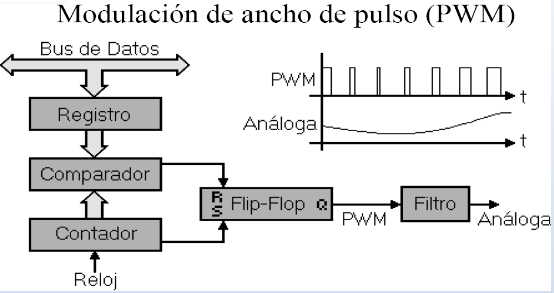
\includegraphics[width=0.6\linewidth]{media/dac-pwm}
	\caption{Conversión D/A mediante PWM}
	\label{fig:dac-pwm}
\end{figure}


\section*{Conversión D/A de entrada paralela}

En los DAC de entrada paralela como se muestra en la figura \ref{fig:dac-entrada-paralela}, el valor digital se presenta simultáneamente en varias líneas (por ejemplo, 8, 10 o 12 bits). Internamente, estos convertidores suelen basarse en redes resistivas R–2R o arquitecturas de fuente de corriente ponderada.

Cada bit controla un interruptor analógico que conecta una resistencia o fuente de corriente a una referencia de voltaje. La suma de todas estas contribuciones genera un voltaje analógico proporcional al valor binario aplicado. La conversión ocurre prácticamente en un solo instante, una vez que el código digital es estable.

% TODO: \usepackage{graphicx} required
\begin{figure}[h]
	\centering
	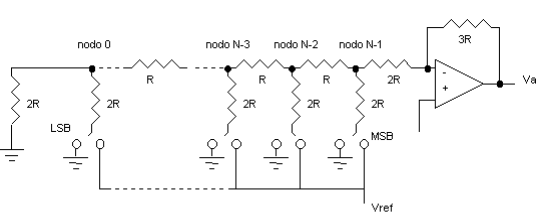
\includegraphics[width=0.7\linewidth]{media/dac-entrada-paralela}
	\caption{Conversor D/A de entrada paralela}
	\label{fig:dac-entrada-paralela}
\end{figure}


Desde la perspectiva del muestreo, el DAC mantiene el valor de salida constante hasta que se aplica un nuevo código, funcionando como un retenedor de orden cero (Zero-Order Hold). Esto es ideal para sistemas donde se requiere baja latencia y alta velocidad de actualización.

\section*{Conversión D/A de entrada serial}
En los DAC seriales, el valor digital se transmite bit a bit a través de un bus de comunicación (SPI, $I^2C$ u otros). Internamente, el DAC posee un registro de desplazamiento que recibe los datos seriales y, una vez completada la palabra digital, transfiere ese valor a la etapa de conversión analógica (generalmente R--2R o corriente conmutada).

Este mecanismo desacopla el proceso de comunicación del proceso de conversión. El muestreo está definido por el momento en que el registro interno del DAC se actualiza, lo que permite una salida estable entre muestras. Muchos DAC incluyen además un \textit{buffer} de salida, mejorando la capacidad de manejo de carga.
